Here you can see how to include an image in your document.

\begin{sidewaysfigure}
\centering
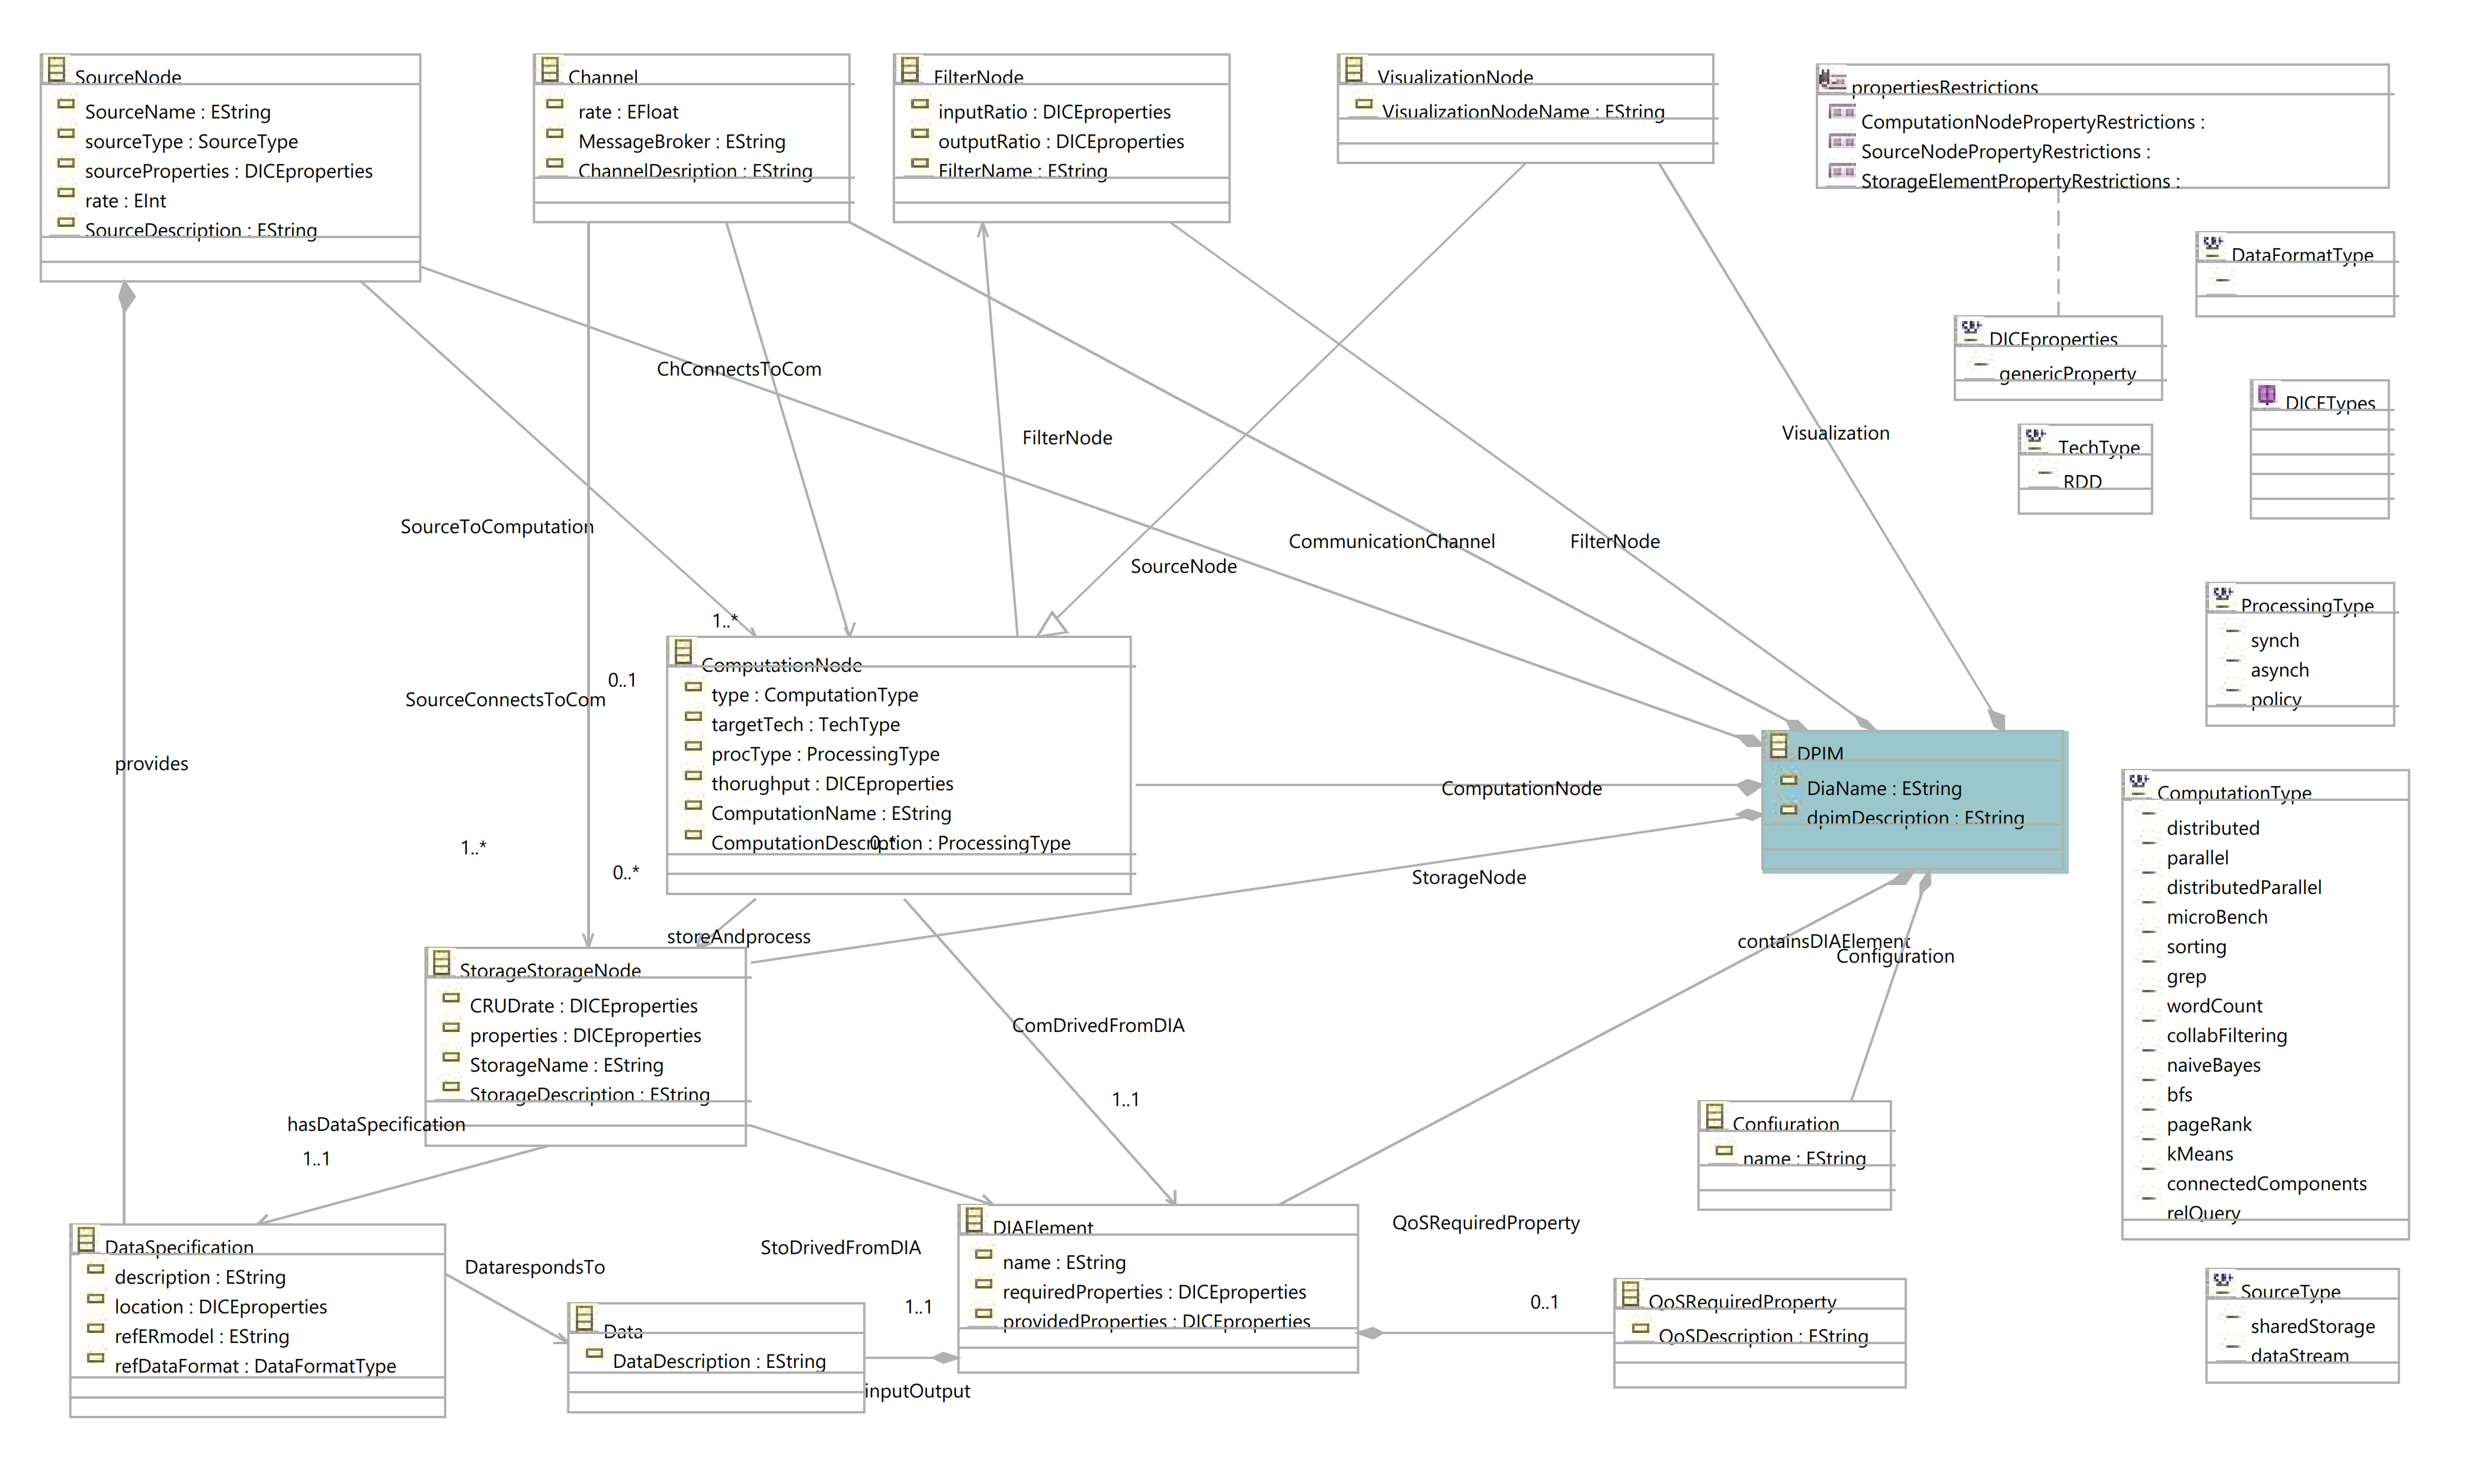
\includegraphics[width=\textwidth]{Images/11.png}
\caption{\label{fig:metamodel}DICE DPIM metamodel.}
\end{sidewaysfigure}

\begin{figure}
\centering
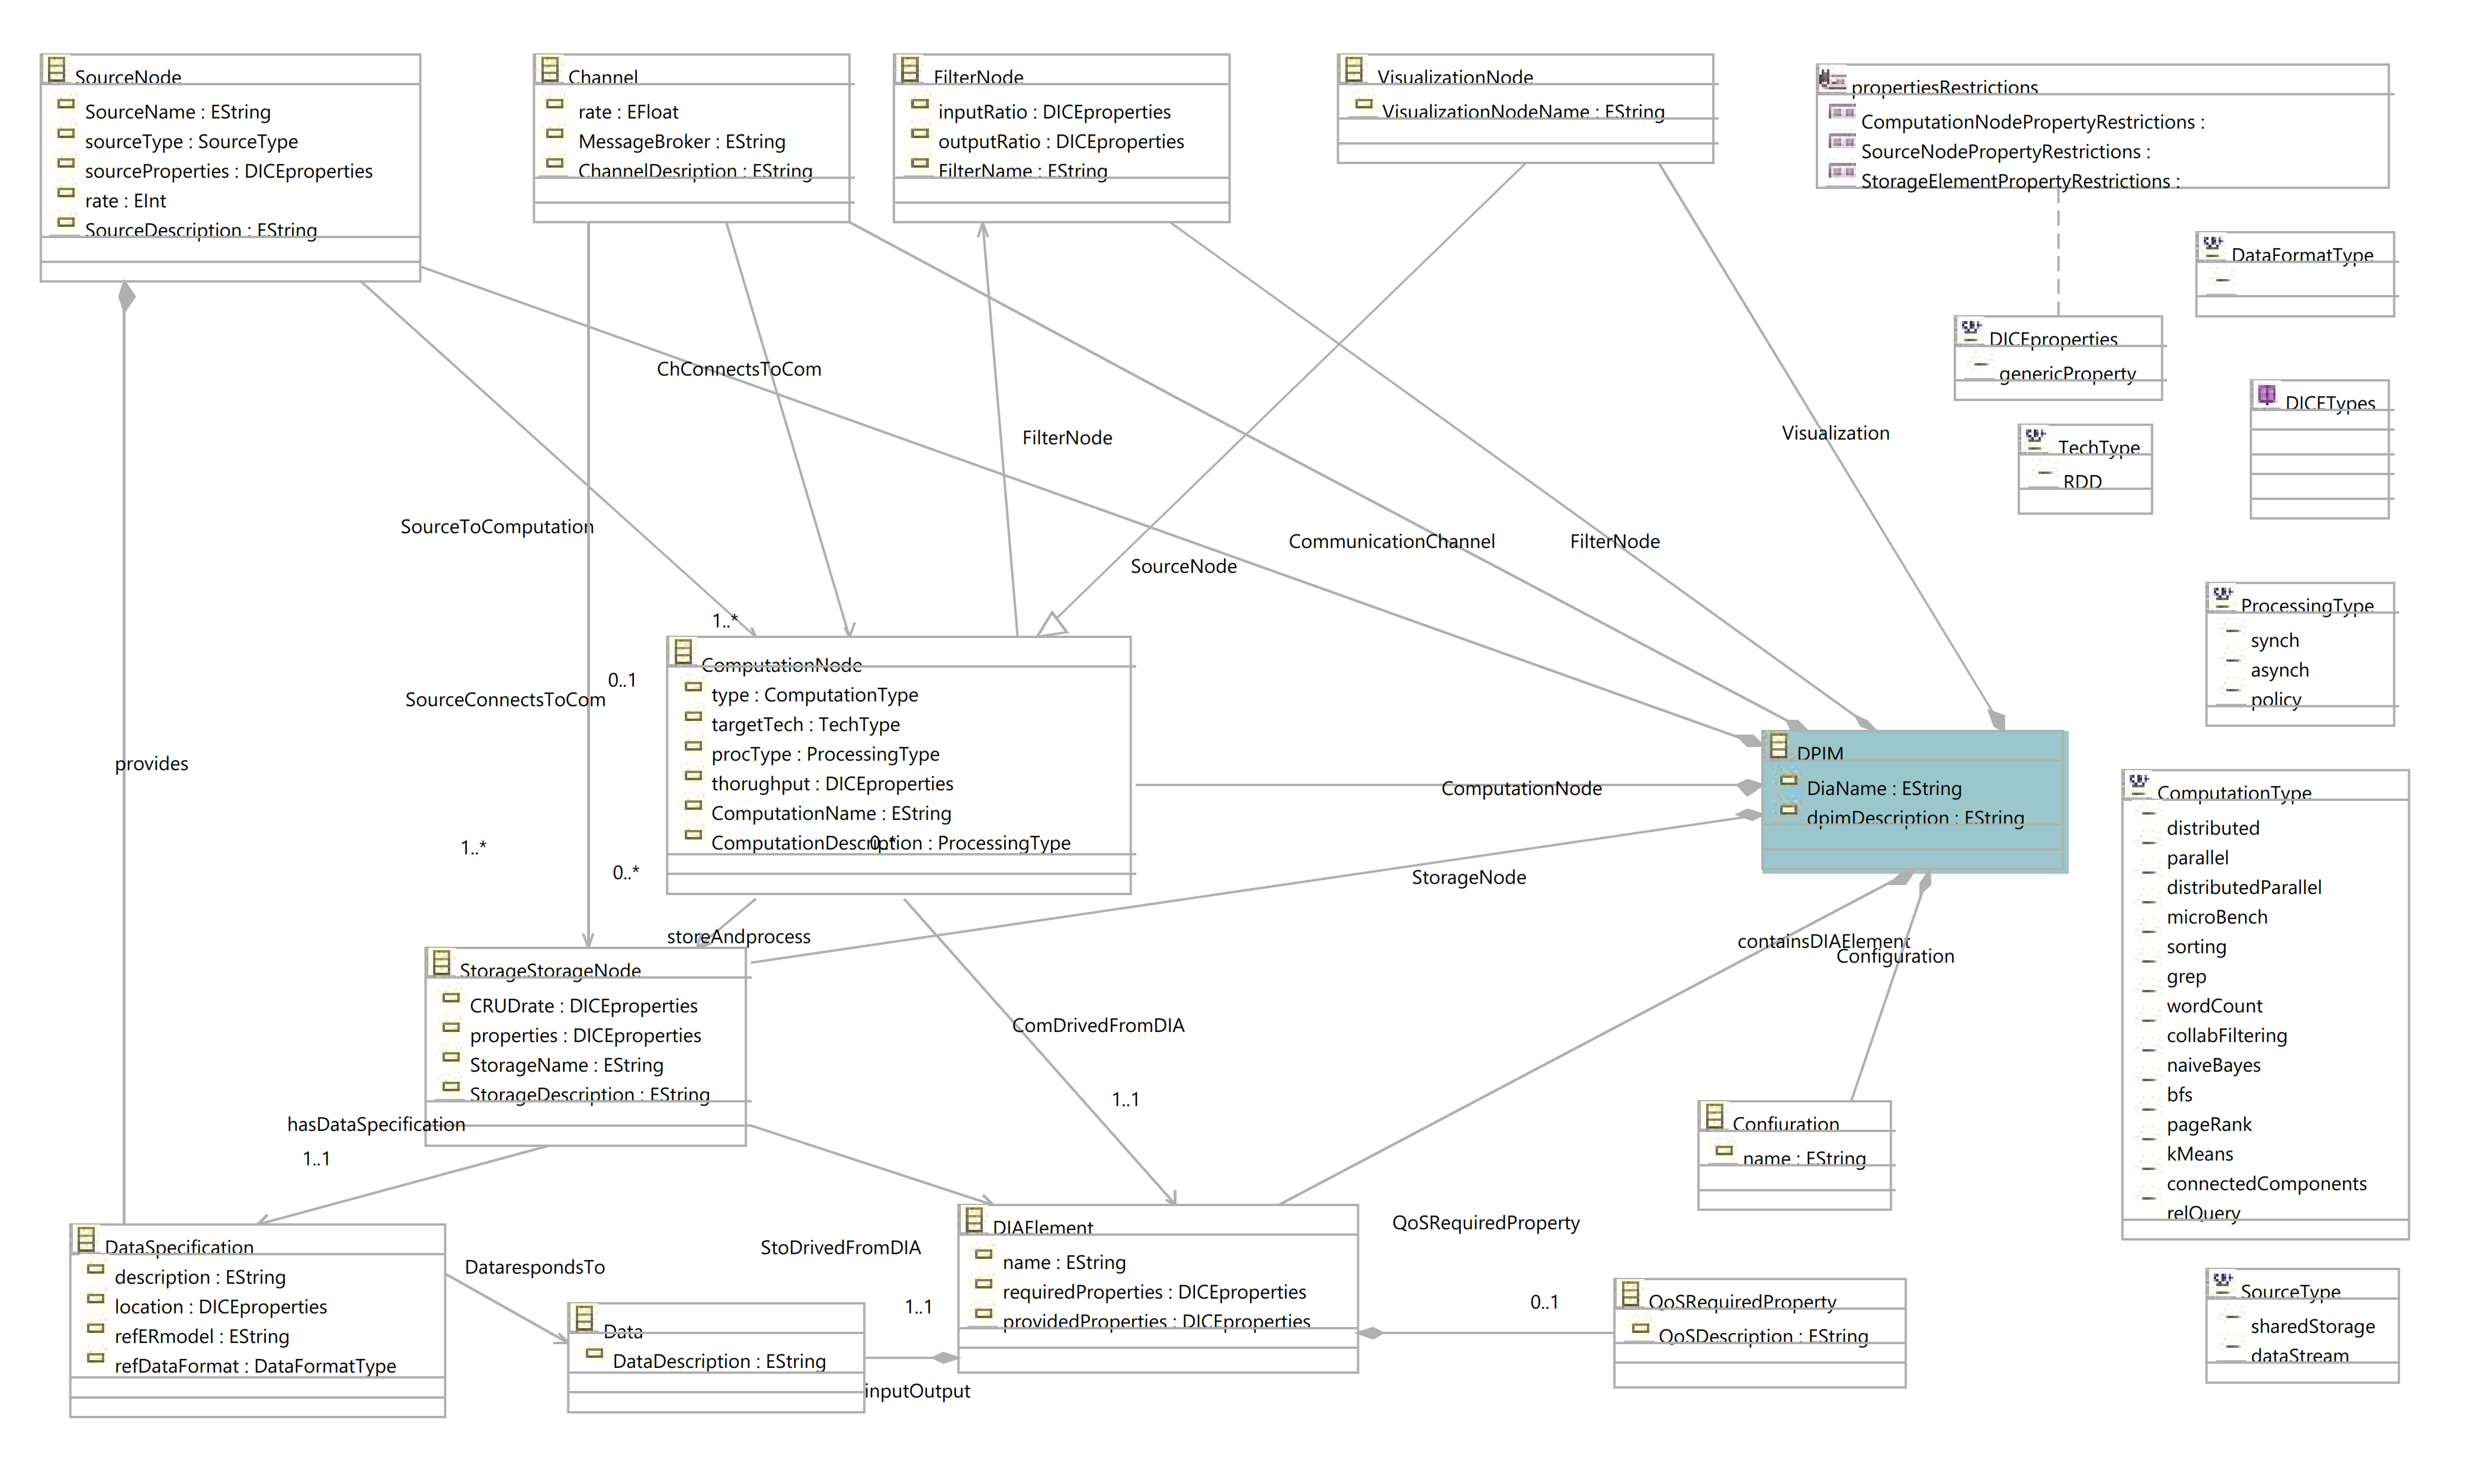
\includegraphics[width=\textwidth]{Images/11.png}
\caption{\label{fig:metamodel2}DICE DPIM metamodel in portrait form.}
\end{figure}

Here is the command to refer to another element (section, figure, table, ...) in the document: \emph{As discussed in Section~\ref{sect:overview} and as shown in Figure~\ref{fig:metamodel}, ...}. Here is how to introduce a bibliographic citation~\cite{DAM}. Bibliographic references should be included in a \texttt{.bib} file. 

Table generation is a bit complicated in Latex. You will soon become proficient, but to start you can rely on tools or external services. See for instance this \href{https://www.tablesgenerator.com}{https://www.tablesgenerator.com}. 

\subsection{Product perspective}
\subsection{Product functions}
the product will be used by farmers, policy makers and agronomists
\subsection{User characteristics}
\subsection{Assumptions, dependencies and constraints}
Assumptions TODO :
\begin{itemize}
	\item
	Cropping seasons are the same on the whole Telengana State and follow the Kharif/Rabi calendar (see Recommended System of Breeder Seed Indent and Supply)
\end{itemize}
\subsubsection{Domain Properties}
here are some domain properties/assumptions
\begin{itemize}
	\item
	DP1 : Every farmer has a smartphone (with geo-tracking,... properties)
	\item
	DP2 : Soil moisture data are updated every 2 days
	\item
	DP : Rainfall conditions are daily updated
	\item
	DP : Rainfall previsions (24/48/72h) are daily updated
	\item
	DP : Data fetched on the different governmental sites are trustworthy reliable
	\item
	DP3 : Farmers are fair when providing data, suggestions and problems
	\item
	DP4 : There are at least 2 farmers and 1 policy maker
	\item
	DP5 : Data from sensors are accurate (in a ... extent)
	\item
	DP6 : Data from the Web are accurate (in a ... extent)
	\item
	DP7 : Sensors are always available, or at least, there is a sufficient number of them to properly describe an area (precision of the DP ?)
	\item
	DP8 : farmers should have received credentials to log in the application
	
\end{itemize}

\subsubsection{use cases}
Here is the diagram for farmers. We suppose they are logged in the application. In case they are not they can simply log in or create an account and then log in.



\begin{table}[htbp]
	\centering
	\begin{tabularx}{\linewidth}{|l|X|}
		\hline
		Name & \multicolumn{1}{c|}{\textit{\textbf{FarmerRegistration}}}                                                   \tabularnewline \hline
		Actors                                               & Farmers                                                    \tabularnewline \hline
		Entry conditions                                              & The farmer is on the DREAM registration form page                                                                                  \tabularnewline \hline
		Event flow                                         & 1.	The system asks for farmer’s data: name, surname, e-mail address, location.                                                                    \tabularnewline 
		& 2.	The farmers fill out the form. The farmer can optionally enable geo-tracking to complete the location field.                                                   \tabularnewline 
		& 3.	The farmer confirms the responses.                                                   \tabularnewline 
		& 4.	The system sends an e-mail containing a validation link to the given e-mail address.                                                \tabularnewline
		& 5.	The system asks the farmer to check his/her e-mail box.                                               \tabularnewline
		& 6.	The farmer clicks on the validation link.                                     \tabularnewline
		& 7.	The system adds the data provided by the farmer to the database.                                  \tabularnewline
		& 8.	Based on the location given by the farmer, the system retrieves the e-mail address of the policy maker dedicated to the farmer newly registered.                               \tabularnewline
		& 9.	The system sends an e-mail to the policy maker to acknowledge that a new farmer has registered.                              \tabularnewline \hline
		Exit conditions & The data are correctly added to the database
		\tabularnewline \hline
		Exceptions & 
		-	The given e-mail address is already in the database. The system displays a message prompting the farmer to modify the dedicated field of the form.  \tabularnewline
		
		&-	The data provided by the farmer have an invalid type or the e-mail address is incorrect. The system displays a message prompting the farmer to modify the dedicated field(s) of the form. 
		\tabularnewline
		&-	There is no registered policy maker dedicated to the area. In that case, no acknowledgement e-mail is sent, but instead a warning message is sent to the developer to urge him/her to contact the adequate policy maker. 
		\tabularnewline
		\hline
	\end{tabularx}   
\end{table}

\begin{table}[htbp]
	\centering
	\begin{tabularx}{\linewidth}{|l|X|}
		\hline
		Name & \multicolumn{1}{c|}{\textit{\textbf{ProductionRelease}}}                                                   \tabularnewline \hline
		Actors                                               & Farmers                                                    \tabularnewline \hline
		Entry conditions                                              & The farmer has begun the cropping season (and eventually finished). \tabularnewline
		&The farmer is already registered on the DREAM platform
		                                                                          \tabularnewline \hline
		Event flow                                         & 1.	The farmer logs in on the platform and clicks on the “Release production data” tab.                                                                   \tabularnewline 
		& 2.	The farmer clicks on the “New release” button                                                   \tabularnewline 
		& 3.	The system displays a form with the following fields: seed variety (to be chosen among a certain list), seed rate, production amount, surface area of the cultivated fields, fertilizer (can be several, to be chosen among a certain list), amount of fertilizer used (one field per fertilizer used), start and end date.                                                 \tabularnewline 
		& 4.	The farmer completes the fields, with respect to the measure units given by the system.                                           \tabularnewline
		& 5.	The farmer confirms.                                               \tabularnewline
		& 6.	The system adds the data to the database.      
		\tabularnewline \hline
		Exit conditions 
		& 
		The data are correctly added to the database
		\tabularnewline \hline
		Exceptions 
		& 
		-	The data provided by the farmer have an invalid type. The system displays a message prompting the farmer to modify the dedicated field(s) of the form
		\tabularnewline
		\hline
	\end{tabularx}   
\end{table}

\begin{table}[htbp]
	\centering
	\begin{tabularx}{\linewidth}{|l|X|}
		\hline
		Name & \multicolumn{1}{c|}{\textit{\textbf{ForumCreation}}}                                                   \tabularnewline \hline
		Actors                                               & Farmers                                                    \tabularnewline \hline
		Entry conditions                                              &
		The farmer is already registered on the DREAM platform
		\tabularnewline
		Event flow                                         & 1.	The farmer logs in on the platform and clicks on the “Forum” tab.                                           \tabularnewline 
		& 2.	The farmer clicks on the “New topic” button.                                            \tabularnewline 
		& 3.	The farmer completes the title and message fields                                            \tabularnewline 
		& 4.	The farmer can optionally add some tags to characterize the topic                                    
		                  \tabularnewline 
		&
		5.	The system adds the topic to the database
		\tabularnewline \hline
		Exit conditions 
		&  The data are correctly added to the database
		\tabularnewline \hline
		Exceptions 
		& 
		-	The data provided by the farmer have an invalid type. The system displays a message prompting the farmer to modify the dedicated field(s) of the form.
		\tabularnewline
		&-	The title or the message is empty. The system displays a message prompting the farmer to fill them both
		
		\tabularnewline
		\hline
	\end{tabularx}   
\end{table}

\begin{table}[htbp]
	\centering
	\begin{tabularx}{\linewidth}{|l|X|}
		\hline
		Name & \multicolumn{1}{c|}{\textit{\textbf{}}}                                                   \tabularnewline \hline
		Actors                                               & Farmers                                                    \tabularnewline \hline
		Entry conditions                                              &
		\tabularnewline
		&
		\tabularnewline \hline
		Event flow                                         &                                            \tabularnewline 
		&                                            \tabularnewline 
		&                                            \tabularnewline 
		&                                     \tabularnewline
		&                                            \tabularnewline
		&                                      \tabularnewline
		&                                 \tabularnewline
		&                               \tabularnewline
		&                               \tabularnewline \hline
		Exit conditions 
		& 
		\tabularnewline \hline
		Exceptions 
		& 
		\tabularnewline
		\hline
	\end{tabularx}   
\end{table}

\begin{figure}
	\centering
	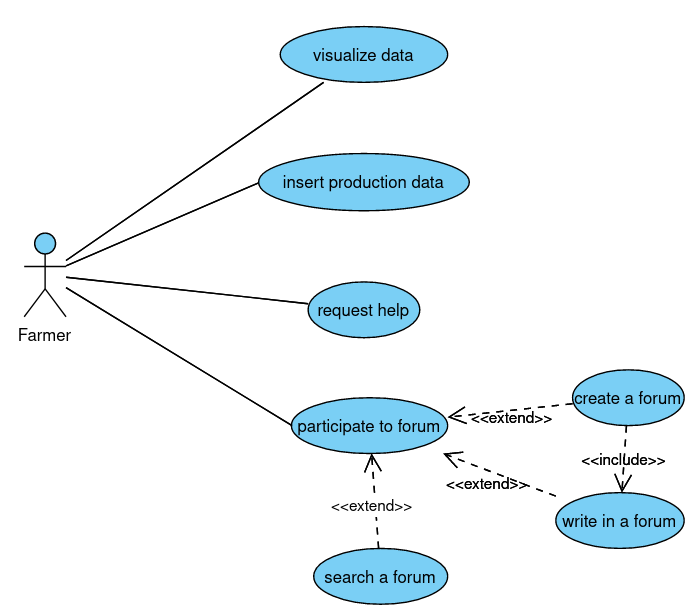
\includegraphics[width=\textwidth]{Images/use-case-farmer.png}
	\caption{\label{fig:usecasefarmer}Use case diagram for logged in farmer}
\end{figure}

\begin{figure}
	\centering
	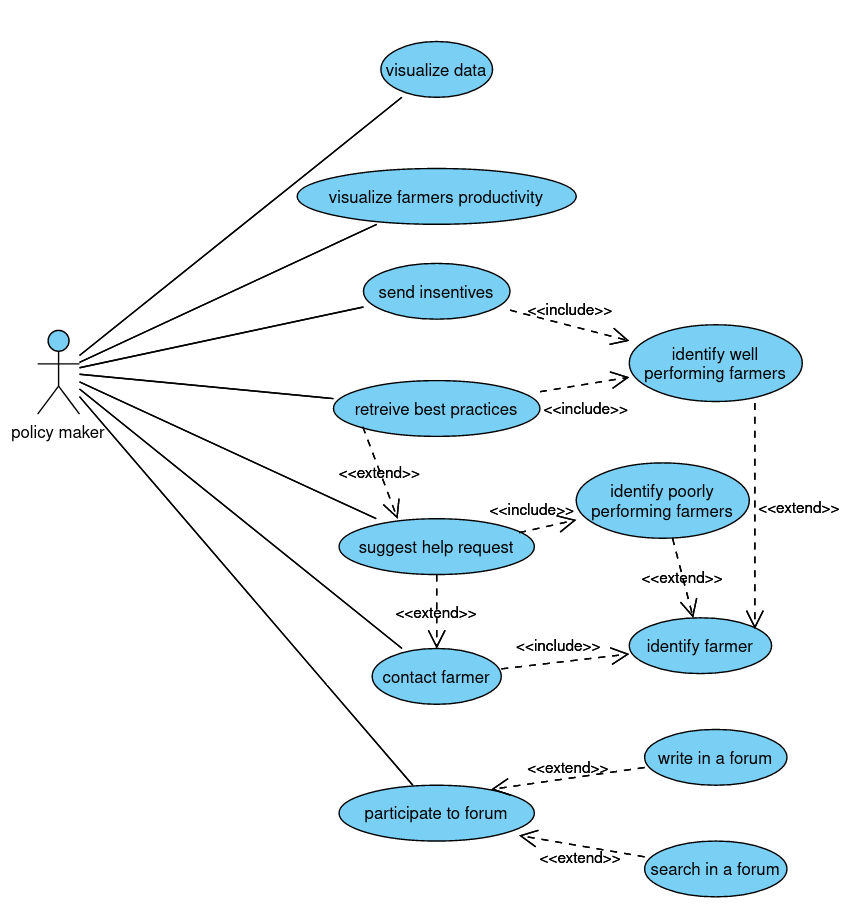
\includegraphics[width=\textwidth]{Images/use-case-policy.png}
	\caption{\label{fig:usecasepolicymakers}Use case diagram for logged in policy makers}
\end{figure}
